% !Tex program = xelatex
\documentclass[UTF8]{ctexart}
\usepackage{hyperref}
\usepackage{graphicx}
\usepackage{listings}
\graphicspath{{./images/}}

\begin{document}
Excerpt of \href{https://yeasy.gitbook.io/docker_practice/}{Docker Practice} by yeasy.
\section{Docker简介}
\subsection{什么是Docker}
Docker 属于 Linux 容器的一种封装,提供简单易用的容器使用接口。它是目前最流行的 Linux 容器解决方案。
Docker 将应用程序与该程序的依赖,打包在一个文件里面。运行这个文件,就会生成一个虚拟容器。程序在这个虚拟容器里运行,就好像在真实的物理机上运行一样。有了 Docker,就不用担心环境问题。

\subsection{Docker优势}
\begin{enumerate}
    \item 更高效的利用系统资源:由于容器不需要进行硬件虚拟以及运行完整操作系统等额外开销,Docker 对系统资源的利用率更高。
    \item 更快速的启动时间:Docker 容器应用,由于直接运行于宿主内核,无需启动完整的操作系统,因此可以做到秒级、甚至毫秒级的启动时间。
    \item 一致的运行环境:Docker 的镜像提供了除内核外完整的运行时环境,确保了应用运行环境一致性。
    \item 持续交付和部署:使用 Dockerfile 使镜像构建透明化,不仅仅开发团队可以理解应用运行环境,也方便运维团队理解应用运行所需条件,帮助更好的生产环境中部署该镜像。
    \item 更轻松的迁移。
    \item 更轻松的维护和扩展:Docker 使用的分层存储以及镜像的技术,使得应用重复部分的复用更为容易,也使得应用的维护更新更加简单,基于基础镜像进一步扩展镜像也变得非常简单。
\end{enumerate}
\begin{figure}[htpb]
    \centering
    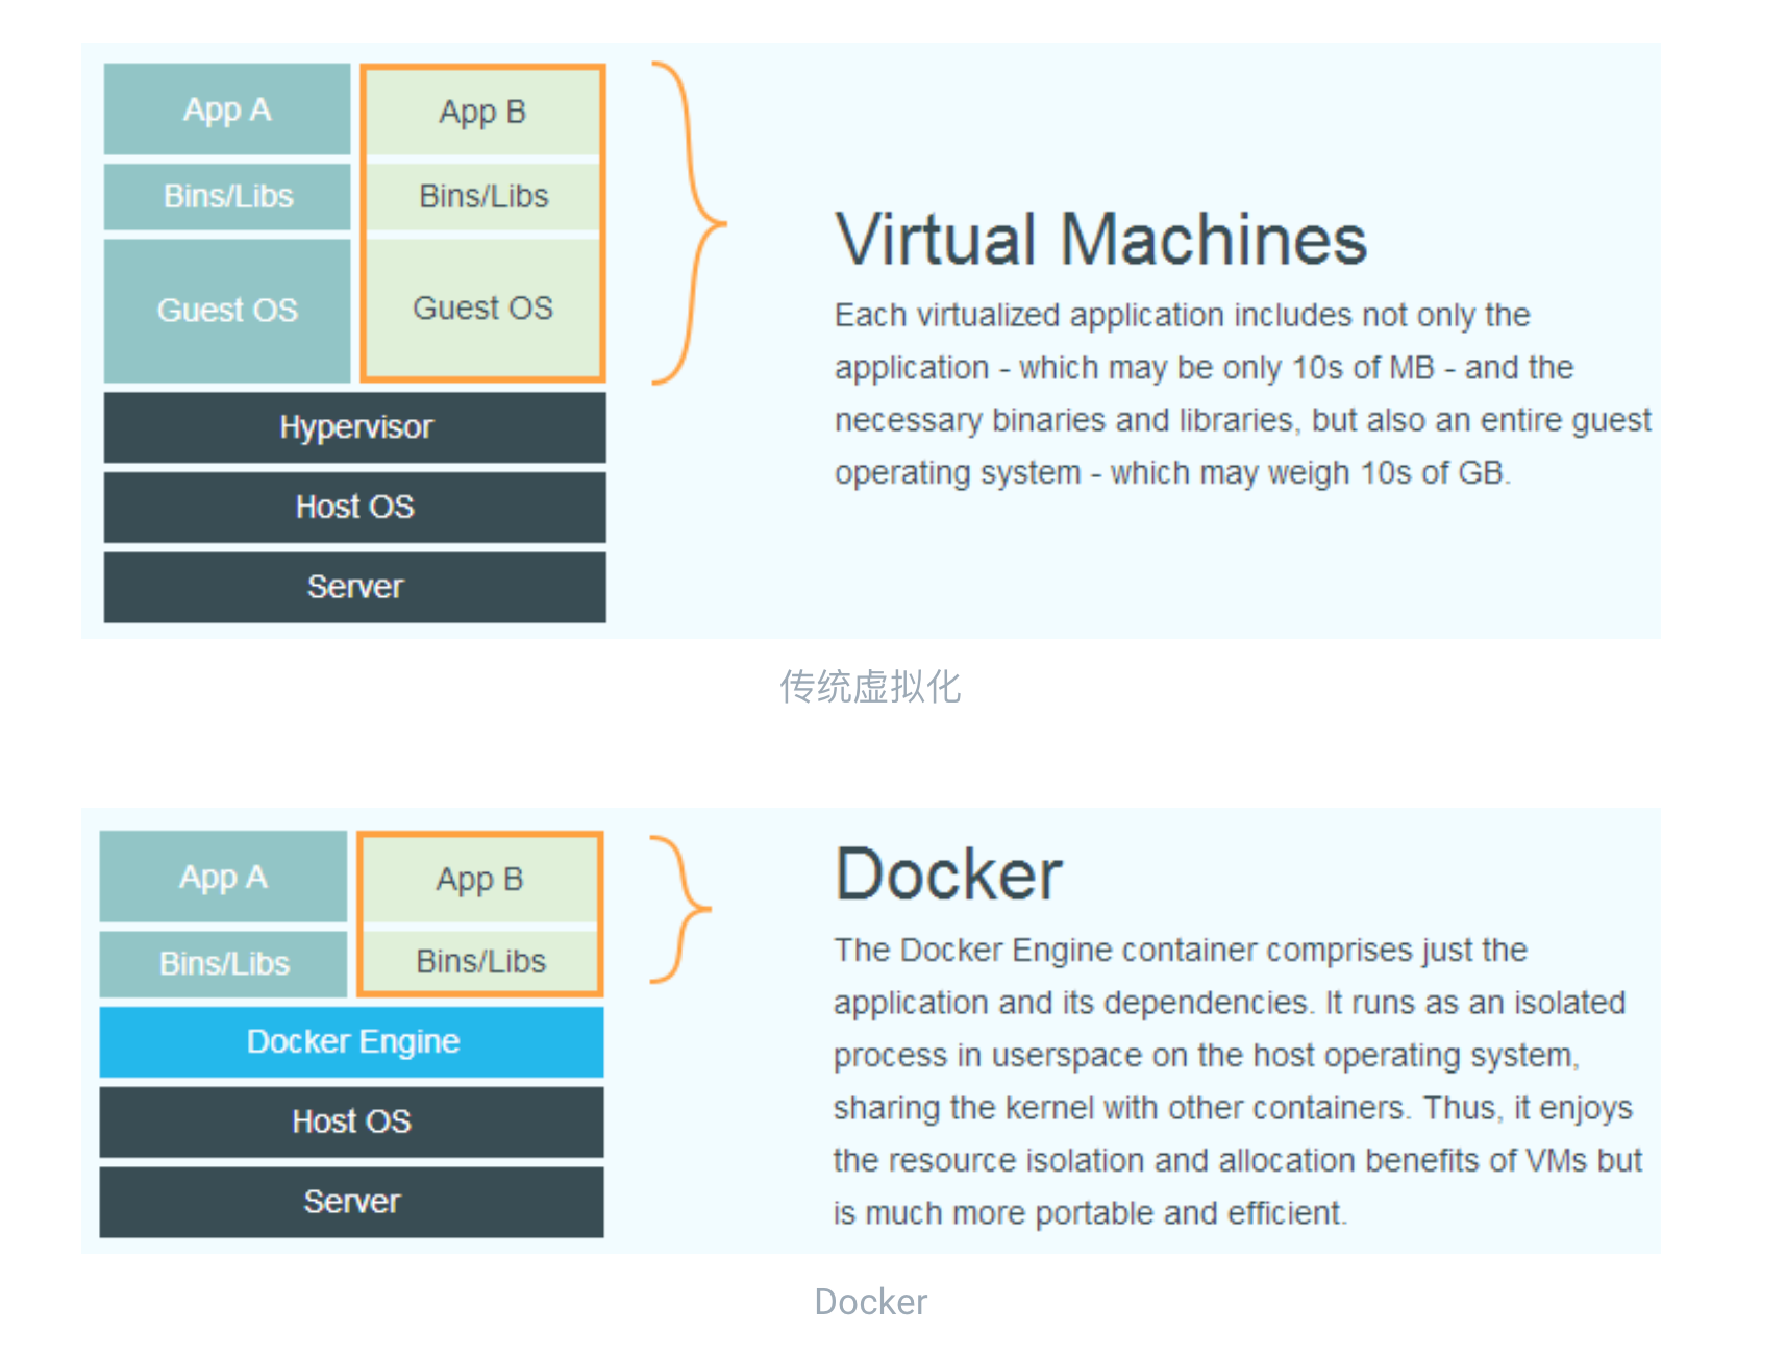
\includegraphics[scale=0.3]{ch1_docker_vs_vm_01.pdf}
    \caption{Docker vs VM 01}
    \label{fig:docker_vs_vm_01}
\end{figure}

\begin{figure}[htpb]
    \centering
    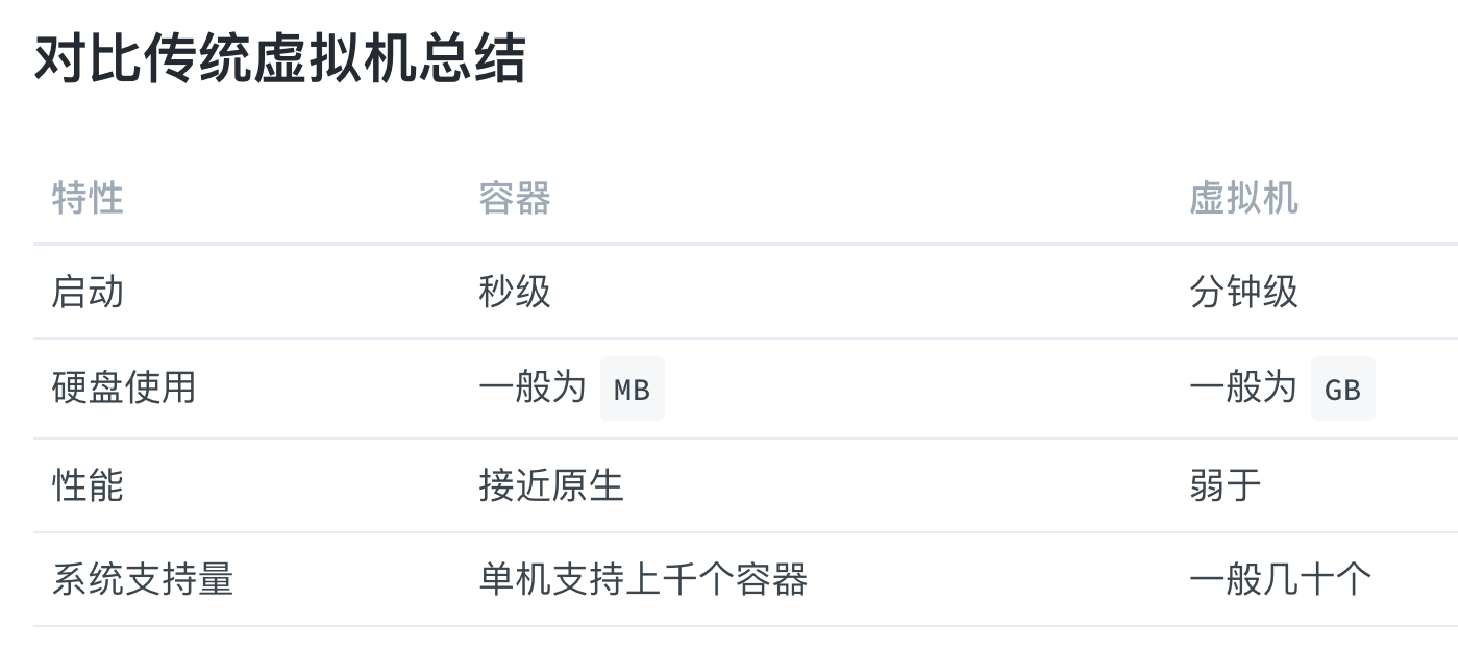
\includegraphics[scale=0.3]{docker_vs_vm_02.pdf}
    \caption{Docker vs VM 01}
    \label{fig:docker_vs_vm_01}
\end{figure}

\section{基本概念}
三个基本概念:
\begin{enumerate}
    \item 镜像(Image)
    \item 容器(Container)
    \item 仓库(Repository)
\end{enumerate}

\subsection{镜像}
操作系统分为内核和用户空间。对于 Linux 而言,内核启动后,会挂载 root 文件系统为其提供用户空间支持。而 Docker 镜像(Image),就相当于是一个 root 文件系统。

Docker 镜像是一个特殊的文件系统,除了提供容器运行时所需的程序、库、资源、配置等文件外,还包含了一些为运行时准备的一些配置参数(如匿名卷、环境变量、用户等)。镜像不包含任何动态数据,其内容在构建之后也不会被改变。
\subsubsection*{分层存储}
镜像只是一个虚拟的概念,其实际体现并非由一个文件组成,而是由一组文件系统组成,或者说,由多层文件系统联合组成。 

镜像构建时,会一层层构建,前一层是后一层的基础。每一层构建完就不会再发生改变,后一层上的任何改变只发生在自己这一层。比如,删除前一层文件的操作,实际不是真的删除前一层的文件,而是仅在当前层标记为该文件已删除。在最终容器运行的时候,虽然不会看到这个文件,但是实际上该文件会一直跟随镜像。因此,在构建镜像的时候,需要额外小心,每一层尽量只包含该层需要添加的东西,任何额外的东西应该在该层构建结束前清理掉。

分层存储的特征还使得镜像的复用、定制变的更为容易。甚至可以用之前构建好的镜像作为基础层,然后进一步添加新的层,以定制自己所需的内容,构建新的镜像。

\subsection{容器}
镜像(Image)和容器(Container)的关系,就像是面向对象程序设计中的 类 和 实例 一样,镜像是静态的定义,容器是镜像运行时的实体。容器可以被创建、启动、停止、删除、暂停等。

容器的实质是进程,但与直接在宿主执行的进程不同,容器进程运行于属于自己的独立的 命名空间。

容器内的进程是运行在一个隔离的环境里,使用起来,就好像是在一个独立于宿主的系统下操作一样。这种特性使得容器封装的应用比直接在宿主运行更加安全。

前面讲过镜像使用的是分层存储,容器也是如此。每一个容器运行时,是以镜像为基础层,在其上创建一个当前容器的存储层,我们可以称这个为容器运行时读写而准备的存储层为 容器存储层。

容器存储层的生存周期和容器一样,容器消亡时,容器存储层也随之消亡。因此,任何保存于容器存储层的信息都会随容器删除而丢失。
按照 Docker 最佳实践的要求,容器不应该向其存储层内写入任何数据,容器存储层要保持无状态化。

所有的文件写入操作,都应该使用 数据卷(Volume)、或者绑定宿主目录,在这些位置的读写会跳过容器存储层,直接对宿主(或网络存储)发生读写,其性能和稳定性更高。
数据卷的生存周期独立于容器,容器消亡,数据卷不会消亡。因此,使用数据卷后,容器删除或者重新运行之后,数据却不会丢失。

\subsection{仓库}
如果需要在其它服务器上使用这个镜像,我们就需要一个集中的存储、分发镜像的服务,Docker Registry 就是这样的服务。

一个 Docker Registry 中可以包含多个 仓库(Repository);每个仓库可以包含多个 标签(Tag);每个标签对应一个镜像。通常,一个仓库会包含同一个软件不同版本的镜像,而标签就常用于对应该软件的各个版本。我们可以通过 <仓库名>:<标签> 的格式来指定具体是这个软件哪个版本的镜像。如果不给出标签,将以 latest 作为默认标签。

仓库名经常以 两段式路径 形式出现,比如 jwilder/nginx-proxy,前者往往意味着 Docker Registry 多用户环境下的用户名,后者则往往是对应的软件名。

\section{安装Docker}
\href{https://yeasy.gitbook.io/docker_practice/install/mac}{参考这里}

\subsection{镜像加速}
\href{https://yeasy.gitbook.io/docker_practice/install/mirror}{参考这里}

\section{使用镜像}
Docker 运行容器前需要本地存在对应的镜像,如果本地不存在该镜像,Docker 会从镜像仓库下载该镜像。

\subsubsection{获取镜像}
从Docker Hub获取:
\begin{lstlisting}
    docker pull [选项] [Docker Registry 地址[:端口号]/]仓库名[:标签]
\end{lstlisting}
Docker 镜像仓库地址:地址的格式一般是 <域名/IP>[:端口号]。默认地址是 Docker Hub。
仓库名:如之前所说,这里的仓库名是两段式名称,即 <用户名>/<软件名>。对于 Docker Hub,如果不给出用户名,则默认为 library,也就是官方镜像。

\subsubsection*{运行}
有了镜像后,我们就能够以这个镜像为基础启动并运行一个容器。e.g. 以 ubuntu:18.04 为例,如果我们打算启动里面的 bash 并且进行交互式操作的话,可以执行下面的命令:
\begin{lstlisting}
    $ docker run -it --rm \
        ubuntu:18.04 \
        bash
\end{lstlisting}
\begin{figure}[htbp]
    \centering
    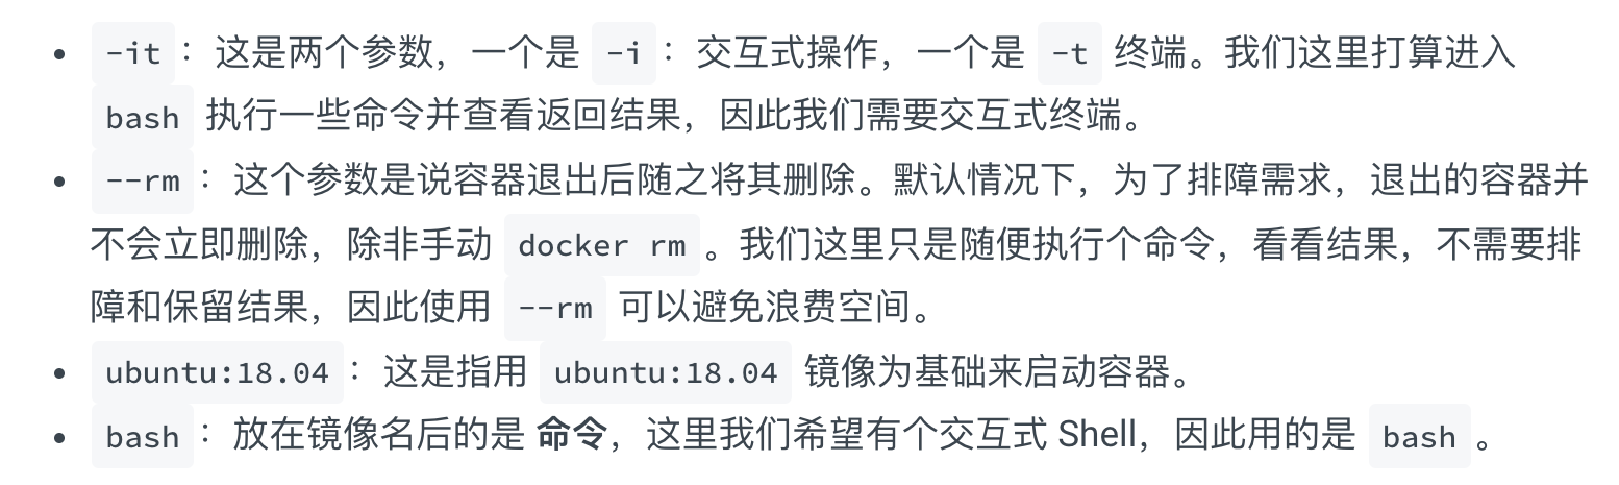
\includegraphics{docker_run_eg.pdf}
    \caption{}
    \label{}
\end{figure}

通过 exit 退出这个容器。
\subsection{列出镜像}
\begin{lstlisting}
    $ docker image ls  # 列出镜像
\end{lstlisting}
列表包含了 仓库名、标签、镜像 ID、创建时间 以及 所占用的空间。镜像 ID 则是镜像的唯一标识,一个镜像可以对应多个 标签。

\subsubsection*{查看空间}
\begin{lstlisting}
    $ docker system df  # 列出所有镜像占用的实际数据卷空间大小
\end{lstlisting}

\subsubsection*{列出部分镜像}
\begin{lstlisting}
    $ docker image ls ubuntu:18.04
    $ docker image ls -f since=mongo:3.2  # -f = --filter 过滤器参数
\end{lstlisting}

\subsubsection*{以特定格式显示}
\begin{lstlisting}
    $ docker image ls -q  # 只列出 ID。结合 docker rm 命令删除镜像
    $ docker image ls --format "{{.ID}}: {{.Repository}}"  # ID + 仓库名
\end{lstlisting}
更多查看 \url{https://yeasy.gitbook.io/docker_practice/image/list}

\subsection{删除镜像}
\begin{lstlisting}
    $ docker image rm [选项] <镜像1> [<镜像2> ...]
\end{lstlisting}
其中,<镜像> 可以是 镜像短 ID、镜像长 ID、镜像名 或者 镜像摘要。

我们可以用镜像的完整 ID,也称为 长 ID,来删除镜像。使用脚本的时候可能会用长 ID,但是人工输入就太累了,所以更多的时候是用 短 ID 来删除镜像。docker image ls 默认列出的就已经是短 ID 了,一般取前3个字符以上,只要足够区分于别的镜像就可以了。

更精确的是使用 镜像摘要 删除镜像。
\begin{lstlisting}
    $ docker image ls --digests 
    $ docker rm <digest>
\end{lstlisting}

\subsubsection*{Untagged 和 Deleted}
如果观察上面这几个命令的运行输出信息的话,你会注意到删除行为分为两类,一类是 Untagged,另一类是 Deleted。我们之前介绍过,镜像的唯一标识是其 ID 和摘要,而一个镜像可以有多个标签。

因此当我们使用上面命令删除镜像的时候,实际上是在要求删除某个标签的镜像。所以首先需要做的是将满足我们要求的所有镜像标签都取消,这就是我们看到的 Untagged 的信息。因为一个镜像可以对应多个标签,因此当我们删除了所指定的标签后,可能还有别的标签指向了这个镜像,如果是这种情况,那么 Delete 行为就不会发生。所以并非所有的 docker image rm 都会产生删除镜像的行为,有可能仅仅是取消了某个标签而已。

当该镜像所有的标签都被取消了,该镜像很可能会失去了存在的意义,因此会触发删除行为。镜像是多层存储结构,因此在删除的时候也是从上层向基础层方向依次进行判断删除。镜像的多层结构让镜像复用变得非常容易,因此很有可能某个其它镜像正依赖于当前镜像的某一层。这种情况,依旧不会触发删除该层的行为。直到没有任何层依赖当前层时,才会真实的删除当前层。

除了镜像依赖以外,还需要注意的是容器对镜像的依赖。如果有用这个镜像启动的容器存在(即使容器没有运行),那么同样不可以删除这个镜像。之前讲过,容器是以镜像为基础,再加一层容器存储层,组成这样的多层存储结构去运行的。因此该镜像如果被这个容器所依赖的,那么删除必然会导致故障。如果这些容器是不需要的,应该先将它们删除,然后再来删除镜像。

\subsubsection*{用 docker image ls 命令来配合}
像其它可以承接多个实体的命令一样,可以使用 docker image ls -q 来配合使用 docker image rm,这样可以成批的删除希望删除的镜像。
\begin{lstlisting}
    $ docker image rm $(docker image ls -q redis)
    $ docker image rm $(docker image ls -q -f before=mongo:3.2)
\end{lstlisting}

\subsection{利用 commit 理解镜像构成}
初学者不必用。慎用! 参考 \url{https://yeasy.gitbook.io/docker_practice/image/commit}

\subsection{使用 Dockerfile 定制镜像}
镜像的定制实际上就是定制每一层所添加的配置、文件。

如果我们可以把每一层修改、安装、构建、操作的命令都写入一个脚本,用这个脚本来构建、定制镜像,那么之前提及的无法重复的问题、镜像构建透明性的问题、体积的问题就都会解决。这个脚本就是 Dockerfile。

Dockerfile 是一个文本文件,其内包含了一条条的 指令(Instruction),每一条指令构建一层,因此每一条指令的内容,就是描述该层应当如何构建。

\subsubsection*{FROM 指定基础镜像}
所谓定制镜像,那一定是以一个镜像为基础,在其上进行定制。就像我们之前运行了一个 nginx 镜像的容器,再进行修改一样,基础镜像是必须指定的。而 FROM 就是指定 基础镜像,因此一个 Dockerfile 中 FROM 是必备的指令,并且必须是第一条指令。

在 Docker Hub 上有非常多的高质量的官方镜像,有可以直接拿来使用的服务类的镜像。如果没有找到对应服务的镜像,官方镜像中还提供了一些更为基础的操作系统镜像。

除了选择现有镜像为基础镜像外,Docker 还存在一个特殊的镜像,名为 scratch。这个镜像是虚拟的概念,并不实际存在,它表示一个空白的镜像。如果你以 scratch 为基础镜像的话,意味着你不以任何镜像为基础,接下来所写的指令将作为镜像第一层开始存在。不以任何系统为基础,直接将可执行文件复制进镜像的做法并不罕见,对于 Linux 下静态编译的程序来说,并不需要有操作系统提供运行时支持,所需的一切库都已经在可执行文件里了,因此直接 FROM scratch 会让镜像体积更加小巧。

\subsubsection*{RUN 执行命令}
RUN 指令是用来执行命令行命令的。由于命令行的强大能力,RUN 指令在定制镜像时是最常用的指令之一。


\end{document}